%% LyX 2.3.6.1 created this file.  For more info, see http://www.lyx.org/.
%% Do not edit unless you really know what you are doing.
\documentclass[english]{article}
\usepackage[T1]{fontenc}
\usepackage[latin9]{inputenc}
\usepackage{geometry}
\geometry{verbose,tmargin=2.5cm,bmargin=2.5cm,lmargin=2.5cm,rmargin=2.5cm}
\usepackage{color}
\usepackage{textcomp}
\usepackage{amstext}
\usepackage{graphicx}
\PassOptionsToPackage{normalem}{ulem}
\usepackage{ulem}

\makeatletter

%%%%%%%%%%%%%%%%%%%%%%%%%%%%%% LyX specific LaTeX commands.
%% Because html converters don't know tabularnewline
\providecommand{\tabularnewline}{\\}

\makeatother

\usepackage{babel}
\begin{document}
{[}SPLIT\_HERE{]}
\begin{enumerate}
\item \textbf{{[}YIJC/PRELIM/9569/2021/P1/Q1{]} }

An iterative function Fn has two parameters, Arr and Object, and returns
an integer. The pseudocode is as follows: 

\noindent\begin{minipage}[t]{1\columnwidth}%
\texttt{01 FUNCTION Fn(Arr: ARRAY, Object: STRING) RETURNS INTEGER }

\texttt{02 \qquad{}Current \textleftarrow{} 1 }

\texttt{03 \qquad{}\qquad{}REPEAT }

\texttt{04 \qquad{}\qquad{}\qquad{}IF Object = Arr{[}Current{]} }

\texttt{05 \qquad{}\qquad{}\qquad{}\qquad{}THEN }

\texttt{06 \qquad{}\qquad{}\qquad{}\qquad{}\qquad{}RETURN Current }

\texttt{07 \qquad{}\qquad{}\qquad{}ENDIF }

\texttt{08 \qquad{}\qquad{}\qquad{}IF Object > Arr{[}Current{]} }

\texttt{09 \qquad{}\qquad{}\qquad{}\qquad{}THEN }

\texttt{10 \qquad{}\qquad{}\qquad{}\qquad{}\qquad{}Next \textleftarrow{}
1 + Current {*} 2 }

\texttt{11 \qquad{}\qquad{}\qquad{}\qquad{}ELSE }

\texttt{12 \qquad{}\qquad{}\qquad{}\qquad{}\qquad{}Next \textleftarrow{}
Current {*} 2 }

\texttt{13 \qquad{}\qquad{}\qquad{}ENDIF }

\texttt{14 \qquad{}\qquad{}\qquad{}Current \textleftarrow{} Next }

\texttt{15 \qquad{}UNTIL Current > LENGTH(Arr) }

\texttt{16 \qquad{}RETURN -1 }

\texttt{17 ENDFUNCTION }%
\end{minipage}A binary search tree is used to store the names of the 12 Chinese
Zodiac animals. The order in which these names were added into the
tree follows the order in the array \texttt{X}. 
\noindent \begin{center}
\begin{tabular}{c|c|cc|c|}
\multicolumn{1}{c}{} & \multicolumn{1}{c}{\texttt{Array X}} &  & \multicolumn{1}{c}{} & \multicolumn{1}{c}{}\tabularnewline
\cline{2-2} \cline{5-5} 
\texttt{X{[}1{]}} & \texttt{'Rat'} &  & \texttt{X{[}7{]}} & \texttt{'Tiger' }\tabularnewline
\cline{2-2} \cline{5-5} 
\texttt{X{[}2{]}} & \texttt{'Monkey'} &  & \texttt{X{[}8{]}} & \texttt{'Dog'}\tabularnewline
\cline{2-2} \cline{5-5} 
\texttt{X{[}3{]}} & \texttt{'Snake'} &  & \texttt{X{[}9{]}} & \texttt{'Horse'}\tabularnewline
\cline{2-2} \cline{5-5} 
\texttt{X{[}4{]}} & \texttt{'Dragon'} &  & \texttt{X{[}10{]}} & \texttt{'Ox'}\tabularnewline
\cline{2-2} \cline{5-5} 
\texttt{X{[}5{]}} & \texttt{'Pig'} &  & \texttt{X{[}11{]}} & \texttt{'Rabbit'}\tabularnewline
\cline{2-2} \cline{5-5} 
\texttt{X{[}6{]}} & \texttt{'Sheep'} &  & \texttt{X{[}12{]}} & \texttt{'Rooster'}\tabularnewline
\cline{2-2} \cline{5-5} 
\end{tabular}
\par\end{center}
\begin{enumerate}
\item Draw the binary tree using the array \texttt{X}. \hfill{}{[}3{]}
\item Complete the trace table templates provided for the following function
calls and state the RETURN value after each function call: 
\noindent \begin{center}
\begin{tabular}{|c|c|c|c|}
\hline 
\texttt{Current } & \texttt{Object = Arr{[}Current{]} } & \texttt{Object > Arr{[}Current{]} } & \texttt{Next }\tabularnewline
\hline 
 &  &  & \tabularnewline
\hline 
 &  &  & \tabularnewline
\hline 
 &  &  & \tabularnewline
\hline 
 &  &  & \tabularnewline
\hline 
\multicolumn{4}{|l|}{\texttt{Output:}}\tabularnewline
\hline 
\end{tabular}
\par\end{center}
\begin{enumerate}
\item Function call: \texttt{Fn(X,'Sheep')} \hfill{}{[}2{]}
\item Function call: \texttt{Fn(X,'Duck')} \hfill{}{[}3{]}
\end{enumerate}
\item Describe the purpose of function \texttt{Fn}. \hfill{}{[}2{]}
\item Explain why this function \texttt{Fn} is more efficient than linear
search.\hfill{} {[}2{]}
\item It is found that one of the Zodiac animals should be named as \textquoteleft Goat\textquoteright{}
instead of \textquoteleft Sheep\textquoteright . Design another array
\texttt{Y} such that the function \texttt{Fn} can be used with the
correct list of the Chinese Zodiac animals. 

Complete the template provided for the array \texttt{Y}.\hfill{}{[}2{]}
\end{enumerate}
\begin{description}
\item [{Template~for~Question~1(b)}]~
\end{description}
\begin{enumerate}
\item[(i)] Function call: \texttt{Fn(X,'Sheep')}

\noindent %
\begin{tabular}{|c|c|c|c|}
\hline 
\texttt{Current} & \texttt{Object = Arr{[}Current{]}} & \texttt{Object > Arr{[}Current{]}} & \texttt{Next}\tabularnewline
\hline 
 &  &  & \tabularnewline
\hline 
 &  &  & \tabularnewline
\hline 
 &  &  & \tabularnewline
\hline 
 &  &  & \tabularnewline
\hline 
\multicolumn{4}{|l|}{\texttt{Output:}}\tabularnewline
\hline 
\end{tabular}
\item[(ii)] Function call: \texttt{Fn(X,'Duck')}
\noindent \begin{flushleft}
\begin{tabular}{|c|c|c|c|}
\hline 
\texttt{Current} & \texttt{Object = Arr{[}Current{]}} & \texttt{Object > Arr{[}Current{]}} & \texttt{Next}\tabularnewline
\hline 
 &  &  & \tabularnewline
\hline 
 &  &  & \tabularnewline
\hline 
 &  &  & \tabularnewline
\hline 
 &  &  & \tabularnewline
\hline 
\multicolumn{4}{|l|}{\texttt{Output:}}\tabularnewline
\hline 
\end{tabular}
\par\end{flushleft}
\end{enumerate}
\begin{description}
\item [{Template~for~Question~1(e)}]~
\end{description}
\noindent \begin{center}
\begin{tabular}{c|c|cc|c|}
\multicolumn{1}{c}{} & \multicolumn{1}{c}{\texttt{Array Y}} &  & \multicolumn{1}{c}{} & \multicolumn{1}{c}{}\tabularnewline
\cline{2-2} \cline{5-5} 
\texttt{Y{[}1{]}} & \texttt{\textcolor{white}{'Rat'}} &  & \texttt{Y{[}7{]}} & \texttt{\textcolor{white}{'Tiger'}}\tabularnewline
\cline{2-2} \cline{5-5} 
\texttt{Y{[}2{]}} & \texttt{\textcolor{white}{'Monkey'}} &  & \texttt{Y{[}8{]}} & \texttt{\textcolor{white}{'Dog'}}\tabularnewline
\cline{2-2} \cline{5-5} 
\texttt{Y{[}3{]}} & \texttt{\textcolor{white}{'Snake'}} &  & \texttt{Y{[}9{]}} & \texttt{\textcolor{white}{'Horse'}}\tabularnewline
\cline{2-2} \cline{5-5} 
\texttt{Y{[}4{]}} & \texttt{\textcolor{white}{'Dragon'}} &  & \texttt{Y{[}10{]}} & \texttt{\textcolor{white}{'Ox'}}\tabularnewline
\cline{2-2} \cline{5-5} 
\texttt{Y{[}5{]}} & \texttt{\textcolor{white}{'Pig'}} &  & \texttt{Y{[}11{]}} & \texttt{\textcolor{white}{'Rabbit'}}\tabularnewline
\cline{2-2} \cline{5-5} 
\texttt{Y{[}6{]}} & \texttt{\textcolor{white}{'Sheep'}} &  & \texttt{Y{[}12{]}} & \texttt{\textcolor{white}{'Rooster'}}\tabularnewline
\cline{2-2} \cline{5-5} 
\end{tabular}
\par\end{center}

{[}SPLIT\_HERE{]}
\item \textbf{{[}YIJC/PRELIM/9569/2021/P1/Q2{]} }

A merge sort algorithm consists of the function \texttt{merge\_sort(seq)}
that takes in an unsorted list \texttt{seq} as an input and returns
a sorted list. The function uses the helper function \texttt{merge(left,right)}
which merges the two sorted lists, \texttt{left} and \texttt{right},
and returns a sorted list. 

The following is the pseudocode for the function \texttt{merge(left,right)}: 

\noindent\begin{minipage}[t]{1\columnwidth}%
\texttt{01 FUNCTION merge(left: LIST, right: LIST) RETURNS LIST }

\texttt{02 \qquad{}IF LENGTH(left) = 0 }

\texttt{03 \qquad{}\qquad{}THEN }

\texttt{04\qquad{}\qquad{}\qquad{} RETURN right }

\texttt{05 \qquad{}\qquad{}ELSE }

\texttt{06\qquad{}\qquad{}\qquad{} IF LENGTH(right) = 0 }

\texttt{07 \qquad{}\qquad{}\qquad{}\qquad{}THEN }

\texttt{08\qquad{}\qquad{}\qquad{}\qquad{}\qquad{} RETURN left }

\texttt{09 \qquad{}\qquad{}\qquad{}ENDIF }

\texttt{10 \qquad{}ENDIF }

\texttt{11 \qquad{}IF left{[}0{]} < right{[}0{]} }

\texttt{12 \qquad{}\qquad{}THEN }

\texttt{13\qquad{}\qquad{}\qquad{} RETURN {[}left{[}0{]}{]} + merge(left{[}1:{]},
right) }

\texttt{14 \qquad{}\qquad{}ELSE }

\texttt{15 \qquad{}\qquad{}\qquad{}RETURN {[}right{[}0{]}{]} +
merge(left, right{[}1:{]}) }

\texttt{16 \qquad{}ENDIF }%
\end{minipage} 
\begin{enumerate}
\item Explain why this is a recursive function. \hfill{}{[}2{]} 
\item State whether this \texttt{merge} implementation is stable or unstable
and explain with an example. \hfill{}{[}2{]} 
\item Complete the merge sort algorithm by writing the pseudocode for the
function \texttt{merge\_sort(seq)}. \hfill{}{[}4{]} 
\item State \textbf{one} advantage and \textbf{one} disadvantage of a merge
sort algorithm over a bubble sort algorithm. \hfill{} {[}2{]} 
\item Explain whether using a merge sort algorithm or a bubble sort algorithm
will be more efficient in arranging the data list \texttt{{[}2,1,3,4,6,5,8,7,9,10,12,11{]}}
in an ascending order. \hfill{}{[}3{]}
\end{enumerate}
{[}SPLIT\_HERE{]}
\item \textbf{{[}YIJC/PRELIM/9569/2021/P1/Q3{]} }

A stack is a last-in-first-out (LIFO) abstract data type (ADT) in
which all the elements are inserted and removed from one end. 

It is common to either use a linked list or an array to implement
a stack
\begin{itemize}
\item In the linked list implementation, a root pointer points to the top
of a stack and a data structure. The data structure contains the value
of the data and a pointer pointing to the next node in the stack. 
\item In the array implementation, a fixed size array is used to store the
elements. 
\end{itemize}
The basic stack operations of \texttt{push()}, \texttt{pop()} and
\texttt{peek()} are provided in both implementations. 
\begin{itemize}
\item \texttt{push()} is used to insert an element into the stack. 
\item \texttt{pop()} removes an element from the stack and returns the value
of the element. 
\item \texttt{peek()} returns the value of the element at the top of the
stack without removing it. 
\end{itemize}
\begin{enumerate}
\item Describe what an abstract data type is and how it benefits the user.\hfill{}
{[}3{]} 
\item State one advantage and one disadvantage of implementing the stack
ADT using a linked list. \hfill{}{[}2{]} 
\item State one advantage and one disadvantage of implementing the stack
ADT using an array.\hfill{} {[}2{]} 
\item Describe how a \texttt{push()} operation is done in a stack ADT which
is implemented using a linked list. \hfill{}{[}3{]} 
\item Describe how the number of elements within a stack can be counted
using only the basic stack operations provided. \hfill{}{[}3{]} 
\end{enumerate}
The following program code uses a Python list as an array with the
built-in functions\texttt{ <list>.insert()} and \texttt{<list>.pop()}. 

\noindent\begin{minipage}[t]{1\columnwidth}%
\texttt{01 def add(seq): }

\texttt{02 \qquad{}stk = {[}{]} }

\texttt{03 \qquad{}def InsertOne(item): }

\texttt{04 \qquad{}\qquad{}if stk=={[}{]} or item < stk{[}0{]}:}

\texttt{05 \qquad{}\qquad{}\qquad{}stk.insert(0,item) }

\texttt{06 \qquad{}else: }

\texttt{07 \qquad{}\qquad{}temp = stk.pop(0) }

\texttt{08 \qquad{}\qquad{}InsertOne(item) }

\texttt{09 \qquad{}\qquad{}stk.insert(0,temp) }

\texttt{10 \qquad{}for ele in seq: }

\texttt{11 \qquad{}\qquad{}InsertOne(ele) }

\texttt{12 \qquad{}return stk }%
\end{minipage}
\begin{enumerate}
\item[(f)] {}
\begin{enumerate}
\item The above is an example of implementing a stack using an array. State
and explain how the program code adds all the elements in the sequence
\texttt{seq} into the stack. \hfill{}{[}2{]} 
\item Modify the above program code such that it uses only the basic stack
ADT operations provided. \hfill{}{[}4{]}
\end{enumerate}
\end{enumerate}
{[}SPLIT\_HERE{]}
\item \textbf{{[}YIJC/PRELIM/9569/2021/P1/Q4{]} }

The following shows a sample of a student\textquoteright s result
slip for the Preliminary Examination. 
\noindent \begin{center}
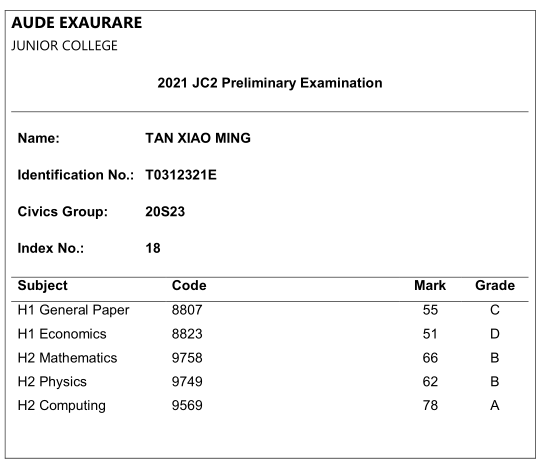
\includegraphics[scale=0.5]{C:/Users/Admin/Desktop/Github/question_bank/LyX/static/img/9569-YIJC-2021-P1-Q4}
\par\end{center}

The college wishes to manage this result information using a relational
database. The normalised database design requires to have a number
of tables. 
\begin{enumerate}
\item Draw an Entity-Relationship (E-R) diagram showing these tables and
the relationships between them. \hfill{}{[}4{]}
\item A table description can be expressed as: 

\texttt{TableName (}\texttt{\uline{Attribute1}}\texttt{, Attribute2{*},
Attribute3, \dots ) }

The primary key is indicated by underlining one or more attributes.
Foreign keys are indicated by using a dashed underline/asterisk. Write
table descriptions for the tables you identified in \textbf{part (a)}.
\hfill{} {[}5{]}
\item Under the Personal Data Protection Act (PDPA), the NRIC/FIN can no
longer be used as a unique identifier for each student. Suggest and
justify a suitable alternative unique identifier for each student.
\hfill{}{[}2{]}
\item Write an SQL query to output the names, civics groups and grades of
students who have obtained at least 60 marks for H2 Computing. \hfill{}{[}4{]}
\end{enumerate}
{[}SPLIT\_HERE{]}
\item \textbf{{[}YIJC/PRELIM/9569/2021/P1/Q5{]} }

The Food Services Industry Digital Plan (IDP) was recently launched
by the Minister of State for Trade and Industry to help F\&B businesses
adopt more digital technologies in their daily operations. The manager
of a Iocal restaurant engaged a consultant to propose a digital solution
for his restaurant operations. 

After conducting a comprehensive study, the consultant proposed a
web-based solution using a client-server model. The solution requires
the following hardware to access the web server wirelessly in the
local area network (LAN): 
\begin{itemize}
\item A tablet device on each table for customers to browse the menu and
order their food items. 
\item Multiple large monitors for the chefs in the kitchen to read the ordered
food items. 
\item A computer station for the service staff to check the table number
before serving the food to the customers. 
\item A computer in the manager\textquoteright s office to update the menu
in the web server and print the daily sales report. 
\end{itemize}
When a customer decides to pay the bill, a QR code will be generated
on the tablet device for him to scan and make online payment using
his personal mobile device.
\begin{enumerate}
\item Explain the meaning of the term client-server model. \hfill{}{[}1{]}
\item Describe the main software components to be developed for the web
server to host this service for the restaurant. \hfill{}{[}2{]}
\item Describe how the customer would use the client tablet device to browse
and order the food items. \hfill{}{[}3{]}
\item Suggest \textbf{one} feature on the digital form that will provide
a positive experience for the customers when using the tablet device
to order their food. Describe the usability principle applied in this
feature. \hfill{}{[}2{]}
\item The manager recommends the proposed solution to the shareholders,
but a number of social issues associated with the solution have been
raised. Describe \textbf{two} possible issues that could have been
raised.\hfill{} {[}2{]}
\end{enumerate}
An alternative to this web-based solution would be to develop a native
application programme for the customers to download and install on
their mobile devices. 
\begin{enumerate}
\item[(f)]  Describe \textbf{one} feature that is only available in the native
application solution and how it is relevant to the solution proposed
for the restaurant. \hfill{}{[}2{]}
\end{enumerate}
The restaurant\textquoteright s manager is also keen to expand his
business to accept online ordering for takeaways. 
\begin{enumerate}
\item[(g)]  Explain \textbf{one} benefit of the web-based solution in this situation.\hfill{}
{[}1{]}
\item[(h)]  Draw the network diagram for the proposed web-based solution and
include all the required hardware for the restaurant to accept online
ordering.\hfill{} {[}5{]}
\item[(i)]  Describe \textbf{two} benefits for the restaurant in implementing
this solution. \hfill{}{[}2{]}
\item[(j)]  For online ordering, the restaurant needs to collect the customer's
name, address and contact number. State and describe \textbf{two}
data protection obligations that the manager needs to comply under
the Personal Data Protection Act. \hfill{}{[}4{]}
\end{enumerate}
{[}SPLIT\_HERE{]}
\item \textbf{{[}YIJC/PRELIM/9569/2021/P1/Q6{]} }

A fantasy card game was developed using object-oriented programming
(OOP) to store its cards\textquoteright{} data. A card can either
be a minion or a weapon. Each card has a name, mana cost, health or
durability and attack power. 

In order to play a card, a player must spend a certain amount of mana
as specified in the card\textquoteright s mana cost. When the card
has been played, the player may decide whether to use it to attack
another minion or not. 

A minion may belong to one of the following races: beast, demon, dragon
or elemental. When a minion is attacked, its health would decrease
according to the attacking card\textquoteright s attack power. Once
the health of a minion decreases to zero, it is destroyed and removed
from the game. 

Instead of health, a weapon has durability and it cannot be attacked.
When a weapon is used for an attack, its durability would decrease
by one. Once the durability of a weapon decreases to zero, it is destroyed
and removed from the game. 
\begin{enumerate}
\item Draw a class diagram, showing: 
\begin{itemize}
\item the base class \texttt{CARD}, 
\item any sub-classes and inheritance from the base class, 
\item the properties for the base class and sub-classes, 
\item appropriate methods with at least one getter and one setter method.\hfill{}
{[}7{]}
\end{itemize}
\item In relation to your diagram in part \textbf{(a)}, explain the terms: 
\begin{enumerate}
\item encapsulation, 
\item inheritance, 
\item polymorphism. \hfill{}{[}6{]}
\end{enumerate}
\item Explain why OOP is a preferred programming paradigm in the development
of this game. \hfill{}{[}2{]}
\end{enumerate}
{[}SPLIT\_HERE{]}
\item \textbf{{[}YIJC/PRELIM/9569/2021/P2/Q1{]} }

During a contact tracing exercise, the TraceTogether token\textquoteright s
tag number, the user\textquoteright s name and the user\textquoteright s
mobile number are stored in an Abstract Data Type (ADT) \texttt{Person}.
The information are stored as a three element tuple as follows: 
\noindent \begin{center}
\texttt{(tag: INTEGER, name: STRING, hp: STRING) }
\par\end{center}

\noindent \begin{center}
\begin{tabular}{|c|c|c|}
\hline 
\textbf{Function } & \textbf{Return Type } & \textbf{Description}\tabularnewline
\hline 
\texttt{make\_person(tag,name,hp) } & \texttt{Person ADT } & A Constructor to create the \texttt{Person} ADT.\tabularnewline
\hline 
\texttt{get\_tag(Person) } & \texttt{INTEGER } & Returns the tag number of the user. \tabularnewline
\hline 
\texttt{get\_name(Person) } & \texttt{STRING } & Returns the name of the user.\tabularnewline
\hline 
\texttt{get\_hp(Person) } & \texttt{STRING } & Returns the mobile number of the user.\tabularnewline
\hline 
\end{tabular}
\par\end{center}

\subsubsection*{Task 1.1 }

Write program code to implement the ADT \texttt{Person} with the above
constructor and accessors.\hfill{} {[}4{]}

\subsubsection*{Task 1.2 }

Write program code for the function \texttt{read\_file()} to read
all the 21 users\textquoteright{} information from the file \texttt{PEOPLE.csv}
and return a list containing all the \texttt{Person} ADTs.\hfill{}
{[}5{]}

\subsubsection*{Task 1.3 }

Write program code for the function \texttt{insertion\_sort(lst)}
that takes the list \texttt{lst} obtained from \textbf{Task 1.2} and
sort them according to their tag numbers in an ascending order using
the insertion sort algorithm.\hfill{} {[}5{]}

Searching for a tag number in a large list of users may be slow and
tedious. However, if the list is sorted, performing a binary search
would be more efficient. 

\subsubsection*{Task 1.4 }

Write program code for the function \texttt{search(lst,num)} that
searches for a tag number \texttt{num} in the sorted list \texttt{lst}
obtained from \textbf{Task 1.3}. The code should 
\begin{itemize}
\item perform a binary search on the sorted list. 
\item return the \texttt{Person} ADT if the tag number \texttt{num} exists.
Otherwise, return \texttt{None}. 
\item print the number of comparisons made in the searching process.\hfill{}
{[}8{]}
\end{itemize}
{[}SPLIT\_HERE{]}
\item \textbf{{[}YIJC/PRELIM/9569/2021/P2/Q2{]} }

Every user is required to carry a tracing token inside an indoor sports
facility so that the sensing device system can detect the token to
read the position of the users and their temperature. The data is
stored as records in the file \texttt{POSRECORDS.txt}, with the following
entries separated by commas: 
\begin{itemize}
\item the tag number (\texttt{INTEGER}) of the tracing token which could
be used to identify the user 
\item the temperature (\texttt{FLOAT}) of the user measured in degree Celsius 
\item the location $(x,y)$\texttt{ (FLOAT,FLOAT)} of the user which consists
of the perpendicular \texttt{x-} and \texttt{y-}distances, measured
in metres, from the walls A and B respectively 
\end{itemize}
The diagram below shows two locations $(x_{1},y_{1})$ and $(x_{2},y_{2})$: 
\noindent \begin{center}
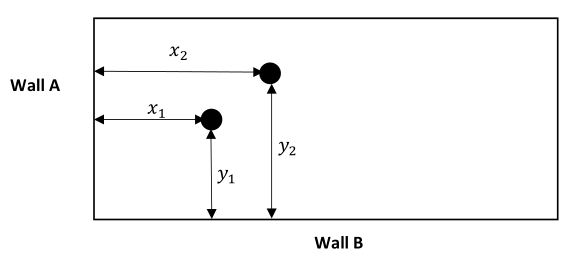
\includegraphics[scale=0.5]{C:/Users/Admin/Desktop/Github/question_bank/LyX/static/img/9569-YIJC-2021-P2-Q2}
\par\end{center}

The distance between two locations can be calculated using the formula: 

\[
\text{Distance}=\sqrt{(x_{2}-x_{1})^{2}+(y_{2}-y_{1})^{2}}
\]


\subsubsection*{Task 2.1 }

Create an empty array \texttt{all\_records} of size 20 and paste the
data from the text file \texttt{POSRECORDS.txt} into your program
code. 

Write program code for the function \texttt{distance(user1,user2)}
that takes in two records and returns the distance between the two
users in metres, correct to 2 decimal places. \hfill{} {[}3{]}

For safety reasons during the Covid-19 pandemic, two users are considered
to be in close proximity if the distance between them is less than
1.5 m apart. 

\subsubsection*{Task 2.2 }

Write program code for the function \texttt{analyse(user1)} that iterates
through all the records in the array \texttt{all\_records}, calculates
the distances between \texttt{user1} and all other users in the array,
and returns a list of tag numbers of the users who are in close proximity
to \texttt{user1}. \hfill{} {[}5{]}

Under the Safe Management Measures, people with a temperature of more
than 37.5 degree Celsius will be flagged out as RED cases and the
people who are in close proximity to these RED cases will be flagged
out as YELLOW cases. The facility manager needs to submit both lists
to the authority daily for follow-up actions. 

\subsubsection*{Task 2.3 }

Write program code for the function \texttt{red\_list(all\_records)}
that iterates through all the records in the array \texttt{all\_records}
and returns a list of tag numbers belonging to the RED cases. \hfill{}
{[}2{]}

\subsubsection*{Task 2.4 }

Write program code for the function \texttt{yellow\_list(red\_cases,all\_records)}
that iterates through all the records in the array \texttt{all\_records}
to check for people who were in close proximity to any of the RED
cases. The function returns a list of tag numbers belonging to the
YELLOW cases. 

Those people flagged out as RED cases in \textbf{Task 2.3} should
not appear in the list of YELLOW cases even though they may be in
close proximity to another RED case. 

You may use the functions written in Task 2.1 and Task 2.2 for the
program code in this task. \hfill{} {[}5{]}

{[}SPLIT\_HERE{]}
\item \textbf{{[}YIJC/PRELIM/9569/2021/P2/Q3{]} }

Shoppe e-Commerce has a mobile application for customers to make purchases
through its online platform. All the customers\textquoteright{} details,
product data and ordering records are kept in the database \texttt{shoppe.db}. 

\subsubsection*{Task 3.1 }

Write program code for the webpage \texttt{index.html} for the customer
to log in to their account. The \texttt{/login} route in the server
code should verify the customer\textquoteright s username and password
using the data in the \texttt{Account} table in the database. 
\noindent \begin{center}
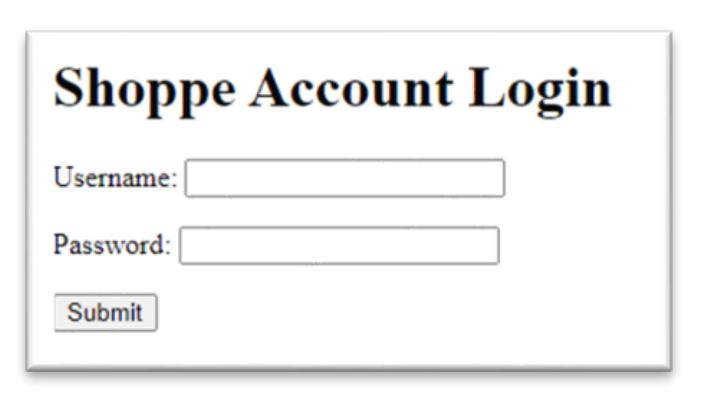
\includegraphics[scale=0.5]{C:/Users/Admin/Desktop/Github/question_bank/LyX/static/img/9569-YIJC-2021-P2-Q3-1}
\par\end{center}

If the log-in details are valid, the customer will receive the webpage
\texttt{display.html}. Otherwise, the customer will be redirected
back to the log-in page. \hfill{} {[}7{]}

\subsubsection*{Task 3.2 }

Write program code for the webpage \texttt{display.html }to display
the customer\textquoteright s details, with the profile picture, and
a menu for the customer to choose the option to update the profile
picture or to check the shopping cart. 
\noindent \begin{center}
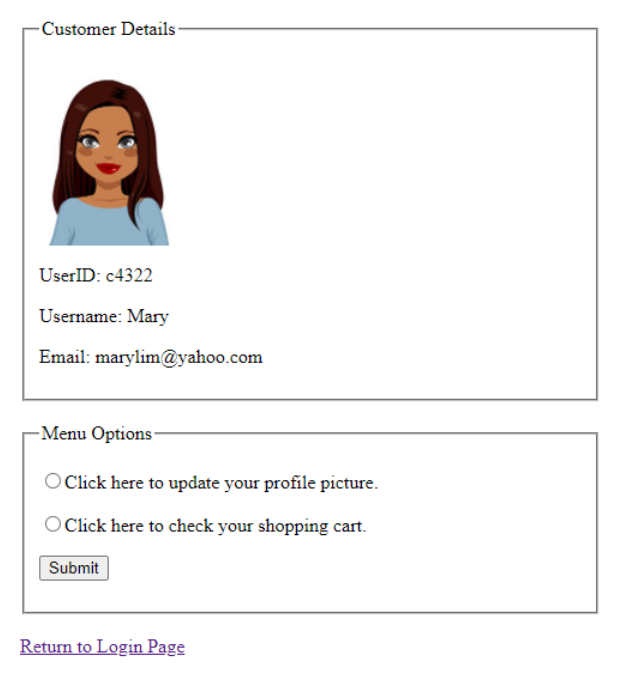
\includegraphics[scale=0.5]{C:/Users/Admin/Desktop/Github/question_bank/LyX/static/img/9569-YIJC-2021-P2-Q3-2}
\par\end{center}

\hfill{} {[}6{]}

A customer, John, does not have a profile picture and he now wishes
to upload the file \texttt{mypic.png}. This picture file will be renamed
as \texttt{John.png} before storing in the web server. 

\subsubsection*{Task 3.3 }

Write program code for the customer to select and upload a picture
file, and it should include the following: 
\begin{itemize}
\item \texttt{/menu} route in the server code to provide the customer with
a webpage \texttt{profile.html} when the option to update the profile
picture is chosen 
\item \texttt{profile.html} to allow the customer to upload a profile picture
in the \texttt{.png} format
\item \texttt{/update} route in the server code to receive the uploaded
picture file and rename it as \texttt{<username>.png} before storing
in the server\textquoteright s \texttt{\textbackslash static\textbackslash photo\textbackslash}
directory 
\item \texttt{success.html} to display a webpage informing the customer
that the profile picture has been successfully uploaded \hfill{}
{[}7{]}
\end{itemize}
The Shoppe customers usually browse through the available products
on the platform and add them to their shopping carts. When they have
decided on their purchase, they will select some or all the items
in the shopping cart before checking out to make payment. 
\noindent \begin{center}
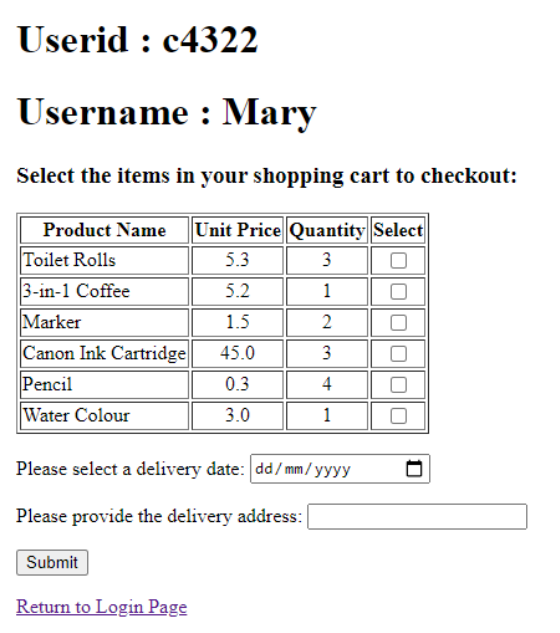
\includegraphics[scale=0.5]{C:/Users/Admin/Desktop/Github/question_bank/LyX/static/img/9569-YIJC-2021-P2-Q3-3}
\par\end{center}

\subsubsection*{Task 3.4 }

Write program code for the customer to select the items to check out
for payment, and it should include the following: 
\begin{itemize}
\item \texttt{/menu} route in the server code to query the \texttt{Cart}
table in the \texttt{shoppe.db} when the customer chooses the option
to check the shopping cart 
\item \texttt{cart.html} to display the list of items in the shopping cart
and let the customer select them for checking out; the customer will
also be required to indicate the preferred date and address for delivery 
\item \texttt{/checkout} route in the server code to receive the customer\textquoteright s
inputs and insert a record into the\texttt{ Orders} table in the\texttt{
shoppe.db }
\item \texttt{success.html} to display the \textbf{total cost} and inform
the customer that the purchase has been successfully recorded.\hfill{}
{[}14{]}
\end{itemize}
{[}SPLIT\_HERE{]}
\item \textbf{{[}YIJC/PRELIM/9569/2021/P2/Q4{]} }

Lessonology is a learning management system that utilises gamification
elements to motivate students to complete their assignments. The Linked
List data structure is used to store the students\textquoteright{}
names and their total experience points. Each node contains a student\textquoteright s
name, the student\textquoteright s total experience points, and a
pointer to the next node. The nodes are linked together according
to the order provided in the \texttt{DATA.txt} file. 

A program is to be written to implement nodes as an instance of the
class \texttt{Node}. The class \texttt{Node} has the following properties
and method: 
\begin{center}
\begin{tabular}{|l|l|}
\hline 
\multicolumn{2}{|c|}{\texttt{Class: Node}}\tabularnewline
\hline 
\multicolumn{2}{|c|}{Properties}\tabularnewline
\hline 
\texttt{\hspace{0.01\columnwidth}}Identifier & \texttt{\hspace{0.05\columnwidth}}Description\tabularnewline
\hline 
\texttt{Name} & The node\textquoteright s value for a student\textquoteright s name.\tabularnewline
\hline 
\texttt{Exp} & The node\textquoteright s value for the student\textquoteright s total
experience points.\tabularnewline
\hline 
\texttt{Pointer} & The pointer to the next node.\tabularnewline
\hline 
\multicolumn{2}{|c|}{Method}\tabularnewline
\hline 
\texttt{\hspace{0.01\columnwidth}}Identifier & \texttt{\hspace{0.05\columnwidth}}Description\tabularnewline
\hline 
\texttt{SetPointer()} & Set the pointer to point at the next node or point to \texttt{None}
when it is the last node.\tabularnewline
\hline 
\end{tabular}
\par\end{center}

A linked list is implemented as an instance of the class \texttt{StudentList}.
The class \texttt{StudentList} has the following property and methods: 
\noindent \begin{center}
\begin{tabular}{|l|l|}
\hline 
\multicolumn{2}{|c|}{\texttt{Class: StudentList}}\tabularnewline
\hline 
\multicolumn{2}{|c|}{Properties}\tabularnewline
\hline 
\texttt{\hspace{0.01\columnwidth}}Identifier & \texttt{\hspace{0.05\columnwidth}}Description\tabularnewline
\hline 
\texttt{Start} & The pointer at the start of the linked list.\tabularnewline
\hline 
\multicolumn{2}{|c|}{Methods}\tabularnewline
\hline 
\texttt{\hspace{0.01\columnwidth}}Identifier & \texttt{\hspace{0.05\columnwidth}}Description\tabularnewline
\hline 
\texttt{Constructor} & Initialise the linked list with the pointer \texttt{Start} assigned
to \texttt{None}.\tabularnewline
\hline 
\texttt{Add()} & Add a new node into the linked list.\tabularnewline
\hline 
\texttt{Update()} & Update the value for the total experience points of a student\textquoteright s
node in the linked list.\tabularnewline
\hline 
\texttt{Delete()} & Delete a node in the linked list.\tabularnewline
\hline 
\texttt{Display()} & Display the current content of the linked list in table form.\tabularnewline
\hline 
\end{tabular}
\par\end{center}

\subsubsection*{Task 4.1 }

Write program code for the classes \texttt{Node} and \texttt{StudentList},
including the \texttt{Constructor},\texttt{ Add() }and \texttt{Display()}
methods. The code should follow the specification given. Do not write
the \texttt{Update()} and \texttt{Delete()} methods yet. 

The \texttt{Add(node)} method for the \texttt{StudentList} class should
add the \texttt{node} containing a student\textquoteright s name and
the student\textquoteright s total experience points to the linked
list, according to the order given in the \texttt{DATA.txt} file. 

Test your code by reading the data from the file \texttt{DATA.txt}
and adding them as nodes into the linked list. The diagram below shows
a portion of the expected output when using the \texttt{Display()}
method on the populated linked list: 
\noindent \begin{center}
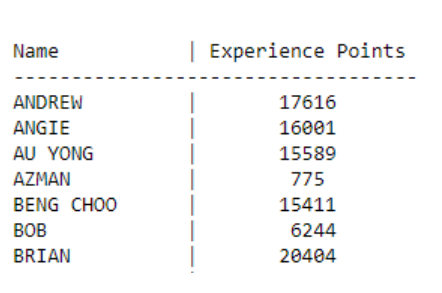
\includegraphics[scale=0.5]{C:/Users/Admin/Desktop/Github/question_bank/LyX/static/img/9569-YIJC-2021-P2-Q4-1}
\par\end{center}

\hfill{}{[}9{]}

\subsubsection*{Task 4.2 }

Each time a student completes an assignment, points will be awarded
and the student\textquoteright s total experience points will be updated. 

Write program code for the \texttt{Update(name,points)} method for
the \texttt{StudentList} class that takes a student\textquoteright s
\texttt{name} and the awarded \texttt{points} as inputs to update
the student\textquoteright s total experience points in the node.
(You may assume that the node containing the student exists in the
linked list.) 

For example, \texttt{Update('BRIAN',100)} will update the total experience
points of a student whose name is \texttt{'BRIAN'} from \texttt{20404}
to \texttt{20504}. \hfill{}{[}3{]}

\subsubsection*{Task 4.3 }

Write program code to implement the \texttt{Delete(name)} method for
the \texttt{StudentList} class to search and remove a node, containing
a particular student\textquoteright s \texttt{name}, in the linked
list. Return \texttt{True} if the node is found and removed; otherwise
return \texttt{False}. (You may assume that the students\textquoteright{}
names are unique in the linked list.) \hfill{}{[}4{]}

\subsubsection*{Task 4.4 }

Another linked list which has pointers linking the nodes in decreasing
order of the experience points is implemented as an instance of the
class \texttt{Leaderboard}. 

The class \texttt{Leaderboard} has the following properties and methods: 
\noindent \begin{center}
\begin{tabular}{|l|l|}
\hline 
\multicolumn{2}{|c|}{\texttt{Class: Leaderboard}}\tabularnewline
\hline 
\multicolumn{2}{|c|}{Properties}\tabularnewline
\hline 
\texttt{\hspace{0.01\columnwidth}}Identifier & \texttt{\hspace{0.05\columnwidth}}Description\tabularnewline
\hline 
\texttt{Start} & The pointer at the start of the linked list.\tabularnewline
\hline 
\multicolumn{2}{|c|}{Methods}\tabularnewline
\hline 
\texttt{\hspace{0.01\columnwidth}}Identifier & \texttt{\hspace{0.05\columnwidth}}Description\tabularnewline
\hline 
\texttt{Constructor} & Inherit the property and all the methods from the class \texttt{StudentList}.
Initialise the linked list with the pointer \texttt{Start} assigned
to \texttt{None}.\tabularnewline
\hline 
\texttt{Add()} & Modify the \texttt{Add()} method in the parent class to add a new
node in decreasing order of total experience points.\tabularnewline
\hline 
\texttt{Update()} & Modify the \texttt{Update()} method in the parent class such that
the linked list is still in decreasing order of experience points
after updating a student\textquoteright s total experience points.\tabularnewline
\hline 
\texttt{DisplayTop()} & Display the content of the nodes in the linked list for the top students
based on their total experience points.\tabularnewline
\hline 
\end{tabular}
\par\end{center}

Write program code for the class \texttt{Leaderboard} to inherit the
properties and methods from the class \texttt{StudentList} with the
modified \texttt{Add()} and \texttt{Update()} methods. The additional
\texttt{DisplayTop(n)} method should display the top \texttt{n} number
of students in the linked list, based on their total experience points.
(You may assume that no two students have the same total experience
points.) 

Test your code by reading the data from the file \texttt{DATA.txt}
and adding them as nodes into this linked list. The diagram below
shows the expected output when using the \texttt{DisplayTop(5)} method
on the linked list: 
\noindent \begin{center}
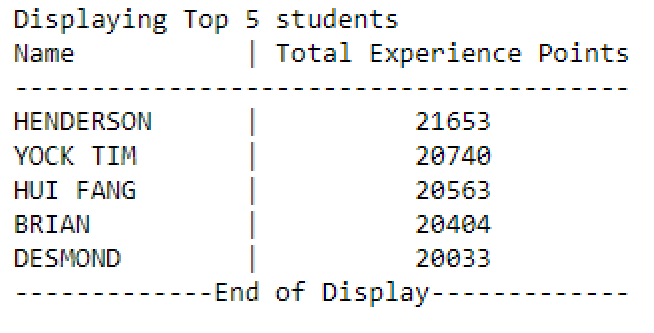
\includegraphics[scale=0.5]{C:/Users/Admin/Desktop/Github/question_bank/LyX/static/img/9569-YIJC-2021-P2-Q4-2}
\par\end{center}

\hfill{}{[}13{]}

{[}SPLIT\_HERE{]}
\end{enumerate}
 
\end{document}
